\documentclass{article}
\usepackage{geometry}
\geometry{top=1.5cm, bottom=2cm, left=2cm, right=2cm}
\usepackage{enumitem}
\usepackage{amsmath}
\usepackage{amsfonts}
\usepackage{graphicx}
\usepackage{physics}
\usepackage{tikz}
\usetikzlibrary{positioning, shapes, arrows.meta}
\newcommand{\od}[1]{\textcolor{blue}{#1}}
\newcommand{\ms}[1]{\textcolor{red}{#1}}
\newcommand{\bb}[1]{\mathbf{#1}}
\newcommand{\m}[1]{\mathcal{#1}}
\usepackage{xcolor}
\usepackage{mathtools}
\usepackage{sectsty}

\usepackage{graphicx} % in your preamble

\usepackage{blindtext}
\usepackage{titlesec}


\usepackage[colorlinks=true, linkcolor=DarkBlue, urlcolor=blue]{hyperref}
\definecolor{DarkBlue}{RGB}{0,0,200}
% SECTION en chiffres romains
\renewcommand\thesection{\Roman{section}}

% SUBSECTION en chiffres arabes
\renewcommand\thesubsection{\arabic{subsection}}
\setcounter{secnumdepth}{2}

% SECTION : plus grand et centré
\titleformat{\section}
  {\normalfont\Large\bfseries \color{DarkBlue}\centering} % style : Large + bold + centré
  {\thesection}{1em}{} % numéro + espacement

% SUBSECTION : un peu plus petit, centré
\titleformat{\subsection}
  {\normalfont\large\bfseries \color{DarkBlue}\centering} % style : Large mais moins que section, centré
  {\thesubsection}{1em}{}

% SUBSUBSECTION : bleu, normal, aligné à gauche
\titleformat{\subsubsection}
  {\normalfont\normalsize\bfseries\color{DarkBlue}\centering} 
  {\thesubsubsection}{1em}{}



\title{Introduction à Git et Github}
\author{Matthieu Vanhoecke}
\begin{document}
\maketitle

\tableofcontents


\section{Commandes de terminal}

Cette section présente les principales commandes du terminal permettant de comparer et de gérer différentes versions d’un code source (Python, C++, \emph{etc.}). Ces outils sont particulièrement utiles pour analyser les modifications apportées à un ou plusieurs fichiers au cours du développement.

\begin{itemize}
    \item \textbf{\texttt{diff Version1.py Version2.py}} : affiche les différences ligne par ligne entre les fichiers \texttt{Version1.py} et \texttt{Version2.py}.  
    Le symbole \texttt{<} indique une ligne présente uniquement dans le premier fichier, tandis que le symbole \texttt{>} indique une ligne présente uniquement dans le second fichier.

    \item \textbf{\texttt{diff -u Version1.py Version2.py}} : génère une sortie au format \emph{unifié}, plus lisible et plus détaillée.  
    Ce format met en évidence le contexte des modifications (par exemple à l’intérieur des boucles, des conditions \texttt{if} ou des fonctions), ce qui facilite l’analyse et la compréhension des changements.

    \item \textbf{\texttt{wdiff Version1.py Version2.py}} : compare les fichiers mot à mot plutôt que ligne par ligne.  
    Contrairement à \texttt{diff}, qui affiche des lignes entières modifiées, \texttt{wdiff} permet d’identifier précisément les mots ajoutés ou supprimés. Cette commande est particulièrement adaptée aux fichiers textuels ou à la documentation.

    \item \textbf{\texttt{diff -u oldfile newfile > change.diff}} : le symbole \texttt{>} redirige la sortie de la commande \texttt{diff} vers le fichier \texttt{change.diff}.  
    Cette commande permet de générer un fichier recensant l’ensemble des modifications entre deux versions. Ce fichier est appelé un \emph{fichier diff} ou \emph{patch}.

    \item \textbf{\texttt{patch fichierpython.py < change.diff}} : applique au fichier \texttt{fichierpython.py} les modifications décrites dans le fichier \texttt{change.diff}.  
    Le symbole \texttt{<} indique que le contenu du fichier \texttt{change.diff} est utilisé comme entrée de la commande \texttt{patch}.  
    Cette méthode fonctionne également sur des répertoires entiers : il est possible de générer un diff sur un ensemble de fichiers, puis d’appliquer les modifications simultanément à un projet contenant des dizaines, voire des centaines de fichiers.

    \item \texttt{ls -la}: affiche tout les fichiers commencant pour un point "." 
\end{itemize}

\subsection{Système de contrôle de versions (VCS)}

Un \emph{Version Control System} (VCS), ou système de contrôle de versions, est un outil permettant de gérer l’évolution de fichiers au cours du temps.
\begin{itemize}
    \item Il permet de stocker du code source, des fichiers de documentation et leurs différentes versions.
    \item Il assure le suivi des modifications apportées aux fichiers, en conservant des informations telles que la date, l’heure et l’auteur des changements.
    \item Les fichiers sont généralement organisés au sein de \texttt{repositories} (dépôts), qui regroupent le code source, la documentation et les fichiers annexes.
    \item Il stocke également les configurations nécessaires au bon fonctionnement des projets.
    \item Un \emph{commit} est un ensemble cohérent de modifications soumis au système de contrôle de versions afin d’être conservé de manière fiable et traçable.
\end{itemize}
\section{Git}
\begin{center}
    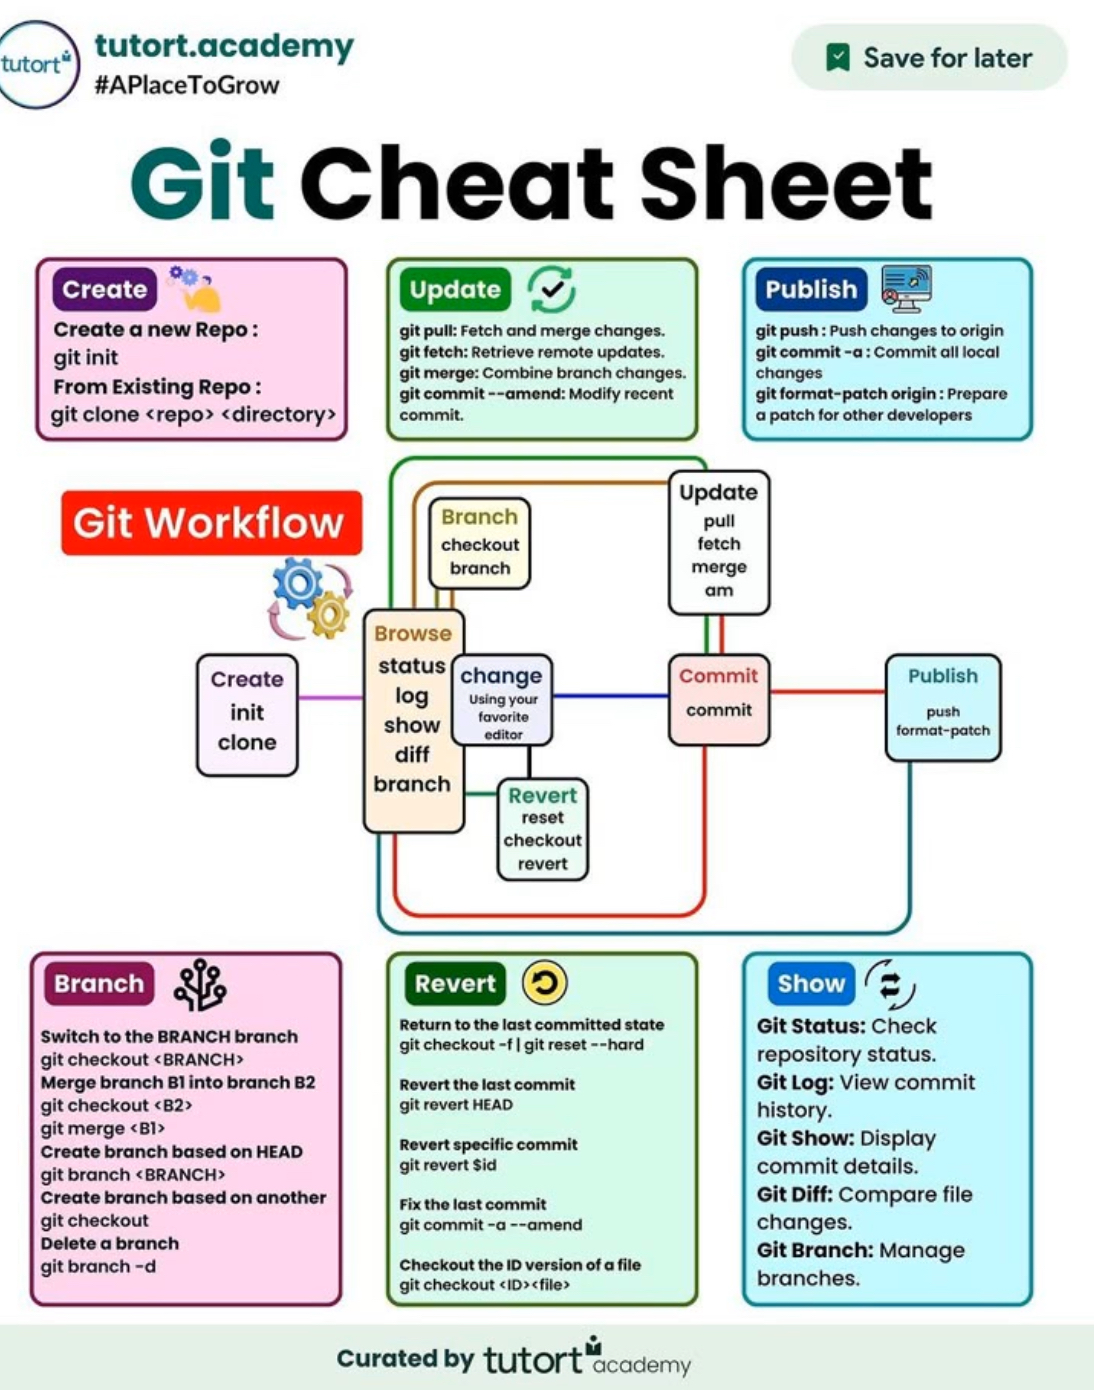
\includegraphics[scale=0.25]{gitsheet.jpeg} 
\end{center}

Git est un système de contrôle de versions \emph{open source}. Il repose sur une architecture distribuée : chaque contributeur d’un dépôt possède une copie complète de l’historique du projet sur sa machine de développement.  
Git peut fonctionner à la fois comme client et comme serveur, et son utilisation ne nécessite pas obligatoirement une connexion à Internet. Il est donc possible de travailler localement, puis de synchroniser les modifications ultérieurement.
\begin{itemize}
    \item Pour connaître la version de Git installée : \texttt{git --version}
\end{itemize}

\subsection{Premiers pas avec Git}
Cette sous-section présente les commandes essentielles pour débuter avec Git, ainsi que les concepts fondamentaux nécessaires à sa bonne utilisation.
\subsubsection{Configuration initiale}
Avant toute utilisation, il est recommandé de configurer Git avec des informations personnelles. Ces informations seront associées à chaque \emph{commit}.
\begin{itemize}
    \item \texttt{git config --global user.email "mail@exemple.com"}
    \item \texttt{git config --global user.name "Mon Nom"}
\end{itemize}
L’option \texttt{--global} indique que ces paramètres s’appliquent à tous les dépôts Git de l’utilisateur sur la machine.
Pour afficher l’ensemble des paramètres de configuration courants, on peut utiliser :
\begin{itemize}
    \item \texttt{git config -l}
\end{itemize}
\subsubsection{Création ou récupération d’un dépôt}
Deux méthodes permettent de commencer à travailler avec Git :
\begin{itemize}
    \item créer un nouveau dépôt local ;
    \item cloner un dépôt existant depuis un serveur distant (abordé ultérieurement).
\end{itemize}
La création d’un nouveau dépôt s’effectue avec la commande :
\begin{itemize}
    \item \texttt{git init}
\end{itemize}
Cette commande initialise un dépôt Git vide dans le répertoire courant.
Le répertoire Git (dossier \texttt{.git}) contient l’ensemble des modifications et leur historique, tandis que l’arborescence de travail (\emph{Working Tree}) contient les versions actuelles des fichiers du projet.

\subsubsection{États des fichiers dans Git}
Dans Git, un fichier peut se trouver dans l’un des trois états suivants :
\begin{itemize}
    \item \textbf{Modifié} : le fichier a été modifié, mais les changements ne sont pas encore suivis par Git.
    \item \textbf{Staged} (zone de transit) : les modifications sont prêtes à être validées.
    \item \textbf{Commit} : les modifications sont enregistrées de manière permanente dans l’historique du dépôt.
\end{itemize}
Le cycle de base est donc :
\begin{center}
\emph{modifié} $\rightarrow$ \emph{staged} $\rightarrow$ \emph{commit}
\end{center}

\subsubsection{Suivi et ajout des fichiers}
Pour que Git commence à suivre un fichier (par exemple \texttt{exemple.py}), celui-ci doit se trouver dans l’arborescence de travail, puis être ajouté à la zone de transit :
\begin{itemize}
    \item \texttt{git add exemple.py}
\end{itemize}
on peut utiliser aussi
\begin{itemize}
    \item \texttt{git add *}
\end{itemize}
pour ajouter tout les fichiers/changement pas dans la zone de transit.
La commande suivante permet de consulter l’état du dépôt à tout moment :
\begin{itemize}
    \item \texttt{git status}
\end{itemize}
Elle indique quels fichiers sont modifiés, suivis, en attente de validation ou déjà enregistrés.

\subsubsection{Visualisation des modifications}
Git fournit plusieurs commandes pour examiner les changements effectués :

\begin{itemize}
    \item \texttt{git diff} : affiche les différences entre les fichiers modifiés et leur dernière version validée (\emph{commit}).  
    Autrement dit, cette commande montre les changements qui ne sont pas encore dans la zone de transit.
    \item \texttt{git diff --staged} : affiche les différences entre les fichiers présents dans la zone de transit et le dernier \emph{commit}.  
    Elle permet donc de vérifier précisément ce qui sera enregistré lors du prochain \emph{commit}.
\end{itemize}

\subsubsection{Validation des modifications (commit)}
Une fois les fichiers ajoutés à la zone de transit, il est nécessaire de valider les modifications à l’aide d’un \emph{commit} :
\begin{itemize}
    \item \texttt{git commit}
\end{itemize}
Cette commande ouvre un éditeur de texte dans lequel l’utilisateur doit saisir un message de \emph{commit}.  
Pour écrire directement le message depuis le terminal, on peut utiliser :

\begin{itemize}
    \item \texttt{git commit -m "Message du commit"}
\end{itemize}
Un bon message de \emph{commit} se compose :
\begin{itemize}
    \item d’une courte description de la modification (environ 50 caractères) ;
    \item éventuellement suivie d’une ligne vide et d’un texte plus détaillé expliquant le changement.
\end{itemize}
Il est également possible de valider directement les fichiers déjà suivis, sans passer explicitement par \texttt{git add} :

\begin{itemize}
    \item \texttt{git commit -a -m "Message du commit"}
\end{itemize}
Cette commande ne fonctionne que pour les fichiers déjà ajoutés au dépôt par le passé. Lors de l’ajout initial d’un fichier, l’utilisation de \texttt{git add} est obligatoire.
\subsection{Interactions avancées avec Git}

\subsubsection{Historique des commits}

Pour consulter l’historique des validations (\emph{commits}) effectuées dans un dépôt, Git met à disposition plusieurs commandes permettant d’obtenir différents niveaux de détail :
\begin{itemize}
    \item \texttt{git log} : affiche la liste des commits, incluant leur identifiant (hash), la date, l’auteur et le message associé.
    \item \texttt{git log -p} : affiche, en complément, les modifications détaillées (\emph{patch}) introduites par chaque commit.
    \item \texttt{git log -n} : affiche uniquement les \emph{n} derniers commits, où \emph{n} est un entier strictement positif.
    \item \texttt{git log --stat} : présente un résumé des changements, indiquant les fichiers modifiés ainsi que le nombre de lignes ajoutées et supprimées.
    \item \texttt{git log --graph --oneline}: pour voir les commits comme un graphes et en une seule ligne par commit.
    \item \texttt{git show \textless{}ID\_commit\textgreater{}} : affiche les informations détaillées et les changements associés à un commit spécifique.
\end{itemize}
On utiliser \texttt{git show} sans l'ID du commit afin de voir les informations concernant le dernier commit.
\subsubsection{Renommer et supprimer des fichiers}

Git permet de gérer explicitement le renommage et la suppression de fichiers tout en assurant le suivi de ces opérations dans l’historique du dépôt :
\begin{itemize}
    \item \texttt{git rm code.py} : supprime le fichier \texttt{code.py} du répertoire de travail et marque cette suppression pour le prochain \emph{commit}.
    \item \texttt{git mv oldname.py newname.py} : renomme le fichier \texttt{oldname.py} en \texttt{newname.py}. Cette commande équivaut à un renommage suivi automatiquement par Git.
\end{itemize}

Toute suppression ou modification du nom d’un fichier doit être validée par un \emph{commit} afin d’être enregistrée dans l’historique du dépôt, par exemple :
\begin{itemize}
    \item \texttt{git commit -m ``Suppression de l'ancien fichier''}
\end{itemize}

Il est également possible d’indiquer à Git d’ignorer certains fichiers (fichiers temporaires, sorties de programme, fichiers générés automatiquement, etc.) à l’aide du fichier \texttt{.gitignore}. Les fichiers listés dans ce fichier ne seront pas suivis par Git.

\subsubsection{Revenir sur des changements et restaurer des fichiers}

Pour annuler les modifications locales effectuées sur un fichier suivi (par exemple \texttt{exemple.py}) et le restaurer dans l’état correspondant au dernier \emph{commit}, la commande suivante peut être utilisée :
\begin{itemize}
    \item \texttt{git checkout NomDuFichier}
\end{itemize}
Cette commande restaure le fichier tel qu’il était lors de la dernière validation, annulant ainsi toutes les modifications locales non validées.

\vspace{0.3cm}

Si un fichier a déjà été ajouté à la zone de transit (\emph{staging area}) à l’aide de \texttt{git add}, il est possible de le retirer de cette zone avec la commande :
\begin{itemize}
    \item \texttt{git reset HEAD NomDuFichier}
\end{itemize}
Cette commande permet de faire revenir le fichier de l’état \emph{staged} à l’état \emph{modifié}, sans perdre les changements effectués.

Pour ces commandes, il est possible d’utiliser le flag :
\begin{itemize}
    \item \texttt{-p}
\end{itemize}
Ce mode interactif permet de sélectionner précisément les parties des modifications à annuler ou à conserver, sans nécessairement revenir en arrière sur l’ensemble des changements.

\subsubsection{Modification d’un commit déjà validé}

Afin de modifier le dernier commit réalisé (ajout de fichiers oubliés, correction du message de commit, etc.), il est possible d’utiliser la commande suivante :
\begin{itemize}
    \item \texttt{git commit --amend}
\end{itemize}
Cette commande crée un nouveau commit en écrasant le commit précédent. Elle permet d’ajouter ou de modifier des fichiers, ainsi que de changer le message du commit, tout en supprimant l’ancien commit de l’historique.

Cette fonctionnalité est particulièrement utile pour corriger rapidement une erreur ou pour inclure des fichiers oubliés. Toutefois, il est fortement déconseillé d’utiliser cette commande dans un dépôt public ou collaboratif, car elle modifie l’historique et peut entraîner des incohérences pour les autres utilisateurs.

\subsubsection{Rollbacks et restauration de commits}

Il est possible d’annuler les effets d’un commit après sa validation en utilisant la commande :
\begin{itemize}
    \item \texttt{git revert HEAD}
\end{itemize}
Cette commande crée un nouveau commit contenant l’inverse exact des changements introduits par le commit ciblé. L’alias \texttt{HEAD} désigne ici le dernier commit effectué.

Pour annuler un commit plus ancien, il est possible de spécifier explicitement son identifiant :
\begin{itemize}
    \item \texttt{git revert \textless{}ID\_commit\textgreater{}}
\end{itemize}

L’identifiant d’un commit est un hash cryptographique calculé à partir de l’ensemble des informations du commit, garantissant la cohérence de l’historique, notamment dans les environnements collaboratifs. En pratique, seuls les 4 à 6 premiers caractères de cet identifiant suffisent généralement pour que Git retrouve le commit correspondant.


\subsection{Création et Fusion de Branches}

\subsubsection{Qu’est-ce qu’une branche}

Une \emph{branche} (\emph{branch}) est un pointeur vers un commit particulier. Plus précisément, elle représente une ligne de développement indépendante au sein d’un projet. Le commit vers lequel une branche pointe correspond au dernier maillon d’une chaîne de commits, c’est-à-dire à l’état le plus récent de cette ligne de développement.

Par défaut, lorsqu’un nouveau dépôt Git est initialisé, Git crée automatiquement une branche principale, traditionnellement nommée \texttt{master} (ou \texttt{main} dans les conventions récentes). Cette branche contient l’historique principal et stable du projet.

L’un des principaux intérêts des branches réside dans leur capacité à isoler le développement. Lorsqu’un développeur souhaite implémenter une nouvelle fonctionnalité, corriger un bug ou expérimenter une idée, il peut créer une branche distincte afin de travailler sans affecter la branche principale. Une fois le développement terminé et validé, il est possible de fusionner (\emph{merge}) cette branche avec la branche principale, intégrant ainsi les changements de manière contrôlée.
Les branches constituent ainsi un mécanisme fondamental de Git, facilitant le travail collaboratif, 
l’expérimentation et la gestion parallèle de plusieurs évolutions du projet.


\subsubsection{Créer de nouvelles branches}

La commande \texttt{git branch} permet de lister, créer, supprimer et manipuler les branches d’un dépôt Git. En particulier, les commandes suivantes sont couramment utilisées :
\begin{itemize}
    \item \texttt{git branch} : affiche la liste des branches du dépôt.
    \item \texttt{git branch nomBranche} : crée une nouvelle branche nommée \texttt{nomBranche}.
\end{itemize}

Lors de l’affichage des branches avec \texttt{git branch}, un astérisque (\texttt{*}) indique la branche actuellement active, c’est-à-dire celle sur laquelle le travail est en cours.

Pour basculer vers une autre branche existante, on utilise la commande :
\begin{itemize}
    \item \texttt{git checkout nomBranche}
\end{itemize}

Il est également possible de créer une nouvelle branche et de s’y positionner immédiatement à l’aide d’une seule commande :
\begin{itemize}
    \item \texttt{git checkout -b nomBranche}
\end{itemize}
Cette commande crée la branche \texttt{nomBranche} et met à jour l’espace de travail pour pointer vers celle-ci.

Après la création d’une branche, le cycle de travail reste identique : il est nécessaire d’ajouter les fichiers modifiés à la zone de transit à l’aide de \texttt{git add}, puis de valider les changements avec un \emph{commit}. Les commits réalisés sur cette branche n’affectent pas les autres branches tant qu’aucune fusion (\emph{merge}) n’est effectuée.

\subsubsection{Visualiser les fichiers dans la branche active}

La commande \texttt{ls -l} permet d’afficher tous les fichiers présents dans le répertoire de travail. Concrètement, elle montre les fichiers correspondant à la **branche actuellement active**, c’est-à-dire celle sur laquelle \texttt{HEAD} pointe.

\begin{itemize}
    \item \textbf{Remarque :} \texttt{ls -l} n’affiche pas les fichiers des autres branches. Pour voir le contenu d’une autre branche, il faut soit changer de branche avec \texttt{git checkout}, soit utiliser une commande Git spécifique comme \texttt{git ls-tree}.
    \item Les fichiers listés comprennent à la fois les fichiers suivis et non suivis présents dans le répertoire de travail. Pour lister uniquement les fichiers suivis par Git, on peut utiliser :
    \begin{itemize}
        \item \texttt{git ls-files}
    \end{itemize}
\end{itemize}


\subsubsection{Interprétation des messages de branche et de \texttt{HEAD}}

Lors de l’exécution de la commande \texttt{git log}, Git affiche non seulement l’historique des commits, mais également des informations sur les branches et la position de \texttt{HEAD}. Ces indications permettent de comprendre rapidement sur quelle branche on travaille et quelles branches pointent vers quels commits.

Dans la sortie de \texttt{git log}, on peut observer des annotations telles que :
\begin{itemize}
    \item \texttt{HEAD} : représente la position actuelle de l’utilisateur dans le dépôt. Il pointe généralement vers la branche active.
    \item \texttt{HEAD -> nomBranche} : indique que \texttt{HEAD} pointe vers la branche \texttt{nomBranche}, ce qui signifie que cette branche est actuellement active.
    \item \texttt{nomBranche} (par exemple \texttt{master}, \texttt{main} ou \texttt{new\_branch}) : indique qu’une branche pointe vers ce commit précis.
\end{itemize}

Par exemple, lorsqu’un commit est effectué sur la branche principale, la sortie de \texttt{git log} peut contenir une ligne similaire à :
\begin{center}
\texttt{HEAD -> master}
\end{center}
Cela signifie que \texttt{HEAD} et la branche \texttt{master} pointent tous deux vers le dernier commit de l’historique.

En revanche, si un commit est réalisé sur une branche secondaire, par exemple \texttt{new\_branch}, la sortie pourra indiquer :
\begin{center}
\texttt{HEAD -> new\_branch}
\end{center}
Dans ce cas, la branche principale (\texttt{master} ou \texttt{main}) continuera de pointer vers un commit plus ancien, ce qui reflète le fait que les nouveaux changements sont isolés dans la branche secondaire.

Ces annotations permettent ainsi de visualiser clairement :
\begin{itemize}
    \item la branche actuellement active,
    \item les branches qui partagent le même commit,
    \item les divergences entre différentes lignes de développement.
\end{itemize}

La compréhension de ces messages est essentielle pour naviguer efficacement dans l’historique d’un dépôt Git et éviter toute confusion lors du travail avec plusieurs branches.
\subsubsection{Suppression d'une branche}

Pour supprimer une branche locale, on utilise la commande suivante :
\begin{itemize}
    \item \texttt{git branch -d nomBranche}
\end{itemize}
Cette commande supprime la branche spécifiée uniquement si tous ses commits ont été fusionnés avec une autre branche.  
Si vous souhaitez forcer la suppression même si la branche n’a pas été fusionnée, vous pouvez utiliser :
\begin{itemize}
    \item \texttt{git branch -D nomBranche}
\end{itemize}

\subsubsection{Fusion de branches (\emph{merging})}

La fusion (\emph{merge}) permet d’intégrer les modifications d’une branche dans une autre. Par exemple, pour fusionner une branche secondaire dans la branche principale, procédez comme suit :

\begin{enumerate}
    \item Basculez sur la branche principale (par exemple \texttt{master} ou \texttt{main}) :
    \begin{itemize}
        \item \texttt{git checkout master}
    \end{itemize}
    \item Fusionnez la branche secondaire dans la branche principale :
    \begin{itemize}
        \item \texttt{git merge nomBrancheASFusionner}
    \end{itemize}
\end{enumerate}

Git tente automatiquement de combiner les changements ligne par ligne. Si les modifications de la branche principale et de la branche secondaire touchent des parties différentes d’un fichier, la fusion se fera automatiquement.

\subsubsection{Gestion des conflits de fusion}

Dans certains cas, Git ne peut pas fusionner automatiquement les branches, généralement lorsque les mêmes lignes d’un fichier ont été modifiées dans les deux branches. Ces situations sont appelées **conflits de fusion**. Voici comment les gérer :

\begin{enumerate}
    \item Git marque les fichiers en conflit et insère des délimitations spéciales dans le fichier pour indiquer les modifications de chaque branche :
    \begin{verbatim}
    <<<<<<< HEAD
    contenu de la branche courante
    =======
    contenu de la branche fusionnée
    >>>>>>> nomBrancheASFusionner
    \end{verbatim}
    \item Il faut alors éditer manuellement le fichier pour résoudre le conflit, en choisissant ou combinant les changements.
    \item Une fois les conflits résolus, ajouter les fichiers à la zone de transit :
    \begin{itemize}
        \item \texttt{git add fichier\_resolu}
    \end{itemize}
    \item Finaliser la fusion avec un commit :
    \begin{itemize}
        \item \texttt{git commit}
    \end{itemize}
\end{enumerate}

\textbf{Remarques :}
\begin{itemize}
    \item Les conflits sont normaux lorsqu’on travaille en parallèle sur plusieurs branches.
    \item Git fournit des outils graphiques et en ligne de commande (\texttt{git mergetool}) pour faciliter la résolution des conflits.
\end{itemize}
Pour interompre la fusion on peut utiliser,
\begin{itemize}
    \item \texttt{git merge --abort}
\end{itemize}
Cela arrete la fusion et reinitialise les fichiers dans chacune des branches.
\subsubsection{Algorithme utilisé lors d'une fusion de branches divergentes}

Lorsque deux branches ont divergé, c’est-à-dire que chacune contient des commits absents de l’autre depuis leur ancêtre commun, Git utilise l’\textbf{algorithme de fusion à trois voies} (\emph{three-way merge}) :

\begin{itemize}
    \item Git identifie le \emph{commit ancêtre commun} (\emph{merge base}) des deux branches.
    \item Il compare les modifications effectuées sur la branche courante (\texttt{HEAD}) et sur la branche à fusionner par rapport à ce commit commun.
    \item Git tente de combiner automatiquement les changements.
    \item Si des modifications affectent les mêmes lignes d’un fichier dans les deux branches, un \textbf{conflit de fusion} se produit, nécessitant une résolution manuelle.
\end{itemize}

\textbf{Remarque :}  
Si la branche courante n’a pas de nouveaux commits depuis la branche à fusionner, Git effectue une \emph{fusion rapide} (\emph{fast-forward}) plutôt qu’une fusion à trois voies.





\newpage
\section{GitHub}

GitHub est un service d’hébergement de dépôts Git. En plus des fonctionnalités de contrôle de version offertes par Git, GitHub fournit des outils supplémentaires tels que le suivi des bogues (\emph{issue tracking}), les wikis, la gestion de projets et la collaboration entre développeurs.  

GitHub permet de partager des dépôts via le Web, de les consulter à distance et de les cloner sur un ordinateur local afin de pouvoir y travailler. D’autres plateformes similaires existent, telles que Bitbucket ou GitLab, qui offrent des fonctionnalités comparables.  

Dans un contexte nécessitant un niveau de sécurité plus élevé ou pour la gestion de données sensibles (notamment en entreprise), il est courant de mettre en place un serveur Git privé, hébergé en interne.

\subsection{Introduction à GitHub}

\subsubsection{Interactions basiques avec GitHub}

Pour créer une copie locale d’un dépôt Git hébergé sur GitHub, on utilise la commande suivante :
\begin{itemize}
    \item \texttt{git clone URL-du-depot}
\end{itemize}
Cette commande clone le dépôt distant sur la machine locale et permet d’utiliser ensuite toutes les commandes Git sur cette copie.

Une fois des modifications effectuées et validées localement à l’aide de \texttt{git commit}, il est possible d’envoyer ces changements vers le dépôt distant avec :
\begin{itemize}
    \item \texttt{git push}
\end{itemize}
Cette commande transmet tous les commits locaux vers le dépôt GitHub correspondant.

\paragraph{Authentification}

Lors des échanges avec un dépôt distant (envoi ou récupération de données), GitHub demande une authentification. Par défaut, celle-ci peut se faire à l’aide d’un identifiant et d’un mot de passe. Il est cependant recommandé d’utiliser une clé SSH pour éviter une authentification répétée et améliorer la sécurité.

Il est également possible d’utiliser un assistant de gestion des identifiants, par exemple :
\begin{itemize}
    \item \texttt{git config --global credential.helper cache}
\end{itemize}
Cette configuration met en cache les identifiants pendant une durée limitée (par défaut 15 minutes).

Pour récupérer les nouvelles modifications présentes sur le dépôt distant et les intégrer à la branche locale courante, on utilise :
\begin{itemize}
    \item \texttt{git pull}
\end{itemize}
Cette commande combine deux opérations : la récupération des nouveaux commits depuis le dépôt distant (\texttt{fetch}) et leur intégration dans la branche locale (\texttt{merge} ou \texttt{rebase}, selon la configuration).



\subsection{Utilisation d’un dépôt distant}

Lorsqu’un dépôt distant est cloné, Git configure automatiquement ce dépôt sous le nom \texttt{origin}. Le terme \texttt{origin} est un \emph{alias} désignant l’URL du dépôt distant à partir duquel le projet a été cloné.  

\paragraph{Signification du terme \texttt{origin}}
\begin{itemize}
    \item Représente le dépôt distant principal.
    \item Permet de référencer facilement le dépôt distant sans retaper l’URL complète.
    \item Il est possible d’avoir plusieurs dépôts distants, chacun avec un nom différent (par exemple \texttt{origin}, \texttt{upstream}, etc.).
\end{itemize}

\paragraph{Commandes pour interagir avec le dépôt distant}
\begin{itemize}
    \item \texttt{git remote -v} : liste les dépôts distants configurés et leurs URL pour \emph{fetch} et \emph{push}.
    \item \texttt{git remote show origin} : fournit des informations détaillées sur les branches suivies et l’état de synchronisation.
    \item \texttt{git branch -r} : affiche uniquement les branches distantes.
    \item \texttt{git status} : indique l’état de la branche locale par rapport à sa branche distante.
\end{itemize}

\subsubsection{Branches locales et distantes après un clone}

Après un clonage, Git configure :
\begin{itemize}
    \item des **branches distantes locales**, par exemple \texttt{origin/master} : copies locales en lecture seule des branches du dépôt distant, reflétant l’état du dépôt GitHub.
    \item des **branches locales**, par exemple \texttt{master} : branches de travail modifiables sur lesquelles tu ajoutes des commits. Elles sont suivies par le pointeur \texttt{HEAD}.
\end{itemize}

\paragraph{Flux de mise à jour et synchronisation}
Pour rester à jour avec le dépôt distant et intégrer les changements :
\begin{enumerate}
    \item \texttt{git fetch} : met à jour les branches distantes locales (\texttt{origin/...}) sans modifier les branches locales.
    \item \texttt{git log origin/master} : permet de visualiser l’historique des commits sur la branche distante.
    \item \texttt{git merge origin/master} ou \texttt{git rebase origin/master} : intègre les changements dans la branche locale.
    \item \texttt{git push} : envoie les commits locaux vers le dépôt distant.
\end{enumerate}

\paragraph{Résumé pratique}
\begin{itemize}
    \item \texttt{origin/master} = reflet du dépôt distant (lecture seule).
    \item \texttt{master} = branche locale modifiable.
    \item \texttt{fetch} et \texttt{git remote update} mettent à jour uniquement les branches distantes locales.
    \item \texttt{merge/rebase} intègre les changements distants dans la branche locale.
    \item \texttt{push} envoie les commits locaux vers GitHub.
\end{itemize}

\subsubsection{Mise à jour d’un dépôt local}

Dans un contexte collaboratif, d’autres contributeurs peuvent ajouter des commits au dépôt distant pendant que l’on travaille localement. Ces modifications ne sont pas automatiquement répercutées dans le dépôt local.  

\paragraph{Vérification de l’état des branches locales et distantes}
\begin{itemize}
    \item \texttt{git remote show origin} : permet de constater si certaines branches locales sont \emph{obsolètes} par rapport aux branches distantes.
\end{itemize}

\paragraph{Récupération des changements}
\begin{itemize}
    \item \texttt{git fetch} : récupère les nouveaux commits depuis le dépôt distant sans modifier la branche locale, mettant à jour uniquement les branches distantes locales.
    \item \texttt{git log origin/master} : permet d’examiner les commits récents sur la branche distante.
    \item \texttt{git status} : indique si la branche locale est en retard ou en avance par rapport à sa branche distante.
\end{itemize}

\paragraph{Intégration des changements}
\begin{itemize}
    \item \texttt{git merge origin/master} : fusionne la branche distante \texttt{origin/master} dans la branche locale. Si la branche locale n’a pas divergé, Git effectue une \emph{fusion rapide} (\emph{fast-forward}).
\end{itemize}

\paragraph{Flux de travail recommandé}
\begin{enumerate}
    \item utiliser \texttt{git fetch} pour examiner les changements sur le dépôt distant,
    \item vérifier leur contenu et leur historique,
    \item utiliser \texttt{git merge} pour intégrer ces changements dans la branche locale.
\end{enumerate}

\paragraph{Récupération et fusion combinées}
La commande \texttt{git pull} combine automatiquement \texttt{fetch} et \texttt{merge} pour mettre à jour la branche locale avec les commits du dépôt distant.

\subsubsection{Mise à jour de tous les dépôts distants : \texttt{git remote update}}

\begin{itemize}
    \item \texttt{git remote update} : met à jour toutes les références de tous les dépôts distants configurés.  
    \item Contrairement à \texttt{git fetch}, qui cible un dépôt ou une branche spécifique, cette commande synchronise toutes les branches distantes pour tous les dépôts distants connus.  
    \item Elle n’affecte pas les branches locales, mais permet d’avoir une vue complète et à jour de l’état des branches distantes avant de faire des fusions ou d’autres opérations.
\end{itemize}



\subsection{Secure Shell (SSH)}

\subsubsection{Définition et objectifs}

Le \emph{Secure Shell} (SSH) est un protocole réseau sécurisé permettant d’accéder à une machine distante via une interface en ligne de commande.  
Il fournit un canal de communication chiffré au-dessus d’un réseau non sécurisé, garantissant :
\begin{itemize}
    \item la confidentialité des données échangées ;
    \item l’intégrité des communications ;
    \item l’authentification des machines et des utilisateurs.
\end{itemize}

SSH est un standard incontournable pour l’administration de serveurs Linux/Unix et pour de nombreuses opérations liées au développement et à la gestion d’infrastructures.

\subsubsection{Notions fondamentales : \emph{shell} et protocole}

Un \emph{shell} est un programme servant d’interface entre l’utilisateur et le système d’exploitation, permettant d’exécuter des commandes.  

Un \emph{protocole} est un ensemble de règles définissant comment deux systèmes communiquent entre eux. Les protocoles réseau sont généralement définis comme des standards ouverts afin de garantir l’interopérabilité entre différents systèmes.

SSH est donc un protocole fournissant un \emph{shell distant sécurisé}.

\subsubsection{Principe de fonctionnement de SSH}

SSH repose sur la cryptographie à clé publique combinée à du chiffrement symétrique :
\begin{itemize}
    \item lors de la première connexion, le serveur SSH envoie sa \textbf{clé publique} au client ;
    \item le client vérifie l’empreinte de cette clé afin de s’assurer de l’identité du serveur ;
    \item le client et le serveur négocient ensuite des algorithmes de chiffrement communs ;
    \item un canal chiffré est établi pour toute la durée de la session.
\end{itemize}

La \textbf{clé privée} du serveur, conservée secrète, est indispensable pour déchiffrer les données.  
Par défaut, un serveur SSH écoute sur le port réseau \texttt{22}.

\subsubsection{Méthodes d’authentification}

SSH propose principalement deux méthodes d’authentification :
\begin{itemize}
    \item \textbf{Authentification par mot de passe} : simple à mettre en place, mais moins sécurisée ;
    \item \textbf{Authentification par clés SSH} : méthode recommandée, plus sécurisée et adaptée à l’automatisation.
\end{itemize}

Une clé SSH est composée d’une paire \emph{clé publique / clé privée}.  
La clé publique peut être copiée sur les serveurs distants, tandis que la clé privée doit rester strictement confidentielle.

\subsubsection{Utilisation de SSH}

\paragraph{Connexion à un serveur distant}
\begin{itemize}
    \item \texttt{ssh utilisateur@hote} : ouvre une session distante sécurisée ;
    \item \texttt{ssh -p port utilisateur@hote} : se connecte via un port SSH spécifique.
\end{itemize}

\paragraph{Génération de clés SSH}
\begin{itemize}
    \item \texttt{ssh-keygen} : génère une paire de clés SSH ;
    \item \texttt{ssh-keygen -t rsa -b 2048} : génère une clé RSA de 2048 bits.
\end{itemize}
Les clés sont stockées par défaut dans le répertoire \texttt{\textasciitilde/.ssh/}.

\paragraph{Installation de la clé publique sur un serveur}
\begin{itemize}
    \item \texttt{ssh-copy-id utilisateur@hote} : copie automatiquement la clé publique sur le serveur distant.
\end{itemize}

\paragraph{Exécution de commandes à distance}
\begin{itemize}
    \item \texttt{ssh utilisateur@hote "commande"} : exécute une commande sans ouvrir de session interactive.
\end{itemize}

\paragraph{Transfert de fichiers sécurisé}
\begin{itemize}
    \item \texttt{scp fichier utilisateur@hote:/chemin} : copie un fichier vers un serveur distant ;
    \item \texttt{sftp utilisateur@hote} : ouvre une session de transfert de fichiers sécurisée.
\end{itemize}

\subsubsection{Fonctionnalités avancées de SSH}

SSH offre plusieurs fonctionnalités avancées :
\begin{itemize}
    \item \textbf{Port forwarding (tunneling)} : redirection sécurisée de ports réseau ;
    \item \textbf{Jump host / bastion} : accès à des serveurs internes via un serveur intermédiaire ;
    \item \textbf{X11 forwarding} : exécution d’applications graphiques distantes avec affichage local.
\end{itemize}

Ces fonctionnalités peuvent être configurées via le fichier \texttt{\textasciitilde/.ssh/config}.

\subsubsection{Configuration du serveur SSH}

Le serveur SSH est fourni par le service \texttt{sshd}.  
Sur les systèmes Linux, son fichier de configuration principal est :
\begin{itemize}
    \item \texttt{/etc/ssh/sshd\_config}
\end{itemize}

Il permet notamment de :
\begin{itemize}
    \item activer ou désactiver l’authentification par mot de passe ;
    \item restreindre les utilisateurs autorisés ;
    \item renforcer la sécurité globale du serveur.
\end{itemize}

\subsubsection{Bonnes pratiques de sécurité}

\begin{itemize}
    \item Ne jamais partager une clé privée SSH.
    \item Protéger les clés privées par une phrase secrète.
    \item Désactiver l’authentification par mot de passe lorsque les clés sont utilisées.
    \item Vérifier toute alerte indiquant un changement de clé du serveur distant.
\end{itemize}

\subsubsection{Synthèse}

SSH est un outil fondamental pour l’administration sécurisée des systèmes.  
Grâce au chiffrement, à l’authentification par clés et à ses nombreuses fonctionnalités, il constitue un pilier de la gestion des infrastructures modernes.


\subsection{API Keys}

\subsubsection{Définition}

Une \emph{API Key} est un jeton d’authentification utilisé par une application pour accéder à une interface de programmation (API).  
Elle permet à un service distant d’identifier le projet ou l’application effectuant une requête et de contrôler les droits associés.

\subsubsection{Authentification et autorisation}

Les API keys remplissent deux fonctions principales :
\begin{itemize}
    \item \textbf{Authentification} : vérifier qu’une application est autorisée à appeler l’API ;
    \item \textbf{Autorisation} : définir quelles ressources ou actions sont accessibles.
\end{itemize}

Contrairement à d’autres mécanismes, une API key identifie généralement une \emph{application} et non un utilisateur individuel.

\subsubsection{Fonctionnement général}

Une API key est :
\begin{itemize}
    \item générée par le fournisseur de l’API ;
    \item envoyée avec chaque requête ;
    \item associée à des permissions et des quotas.
\end{itemize}

Elle peut être transmise :
\begin{itemize}
    \item via un paramètre d’URL ;
    \item via un en-tête HTTP (méthode recommandée) ;
    \item plus rarement via un endpoint dédié.
\end{itemize}

\subsubsection{Cas d’usage}

Les API keys sont adaptées pour :
\begin{itemize}
    \item bloquer l’accès anonyme à une API ;
    \item limiter le nombre de requêtes ;
    \item analyser les usages et statistiques ;
    \item filtrer les journaux par application.
\end{itemize}

\subsubsection{Limites}

Les API keys ne doivent pas être utilisées pour :
\begin{itemize}
    \item identifier précisément des utilisateurs ;
    \item fournir une autorisation fine et hautement sécurisée ;
    \item protéger seules des données sensibles.
\end{itemize}

Des solutions comme \emph{OAuth} sont préférables pour ces usages.

\subsubsection{Bonnes pratiques de sécurité}

\begin{itemize}
    \item Ne jamais inclure une API key dans un dépôt public.
    \item Utiliser des variables d’environnement pour les stocker.
    \item Restreindre permissions et quotas.
    \item Régénérer régulièrement les clés compromises.
\end{itemize}

\subsubsection{Synthèse}

Les API keys constituent un mécanisme simple et efficace pour contrôler l’accès aux API.  
Elles doivent cependant être utilisées avec prudence et combinées à des mécanismes plus robustes lorsque la sécurité est critique.




\subsection{Résolution des conflits}

\subsubsection{ Le Pull-Merge-Push}
Dans un environnement collaboratif, il est fréquent que plusieurs personnes modifient le même dépôt en parallèle. Un conflit peut survenir lorsque l’on tente d’envoyer (\texttt{push}) des modifications locales alors que de nouveaux commits ont déjà été ajoutés sur le dépôt distant (GitHub) par un autre collaborateur.

\paragraph{Origine des conflits}
Lorsque Git détecte que la branche locale est en retard par rapport à la branche distante, il refuse le \texttt{push} afin d’éviter d’écraser le travail des autres. Un message d’erreur indique alors que la branche distante contient des modifications inconnues localement.

\paragraph{Synchronisation avec le dépôt distant}
Dans ce cas, il est nécessaire de synchroniser d’abord le dépôt local avec le dépôt distant en utilisant :
\begin{itemize}
    \item \texttt{git pull}
\end{itemize}
Cette commande récupère les nouveaux commits du dépôt distant et tente de les fusionner avec la branche locale courante.

\paragraph{Gestion des conflits de fusion}
Si Git ne parvient pas à fusionner automatiquement les modifications (par exemple lorsque les mêmes lignes d’un fichier ont été modifiées), il signale un \emph{conflit de fusion}. Les fichiers concernés sont alors marqués comme conflictuels et doivent être corrigés manuellement par le développeur.  
Une fois les conflits résolus, il faut :
\begin{itemize}
    \item ajouter les fichiers corrigés avec \texttt{git add},
    \item valider la fusion avec \texttt{git commit}.
\end{itemize}

\paragraph{Visualisation de l’historique des commits}
Pour visualiser l’arbre des commits sur l’ensemble des branches (locales et distantes), on peut utiliser :
\begin{itemize}
    \item \texttt{git log --graph --oneline --all}
\end{itemize}
Cette commande permet de mieux comprendre l’historique du projet et les divergences entre branches.

\paragraph{Inspection des changements}
Pour examiner précisément les modifications introduites par les commits d’une branche distante, on peut utiliser :
\begin{itemize}
    \item \texttt{git log -p origin/master}
\end{itemize}
Cette commande affiche le détail des changements ligne par ligne, ce qui est utile pour analyser les modifications avant ou après une fusion.

\paragraph{Résumé}
En cas de conflit lors d’un \texttt{push}, il est essentiel de :
\begin{itemize}
    \item synchroniser le dépôt local avec \texttt{git pull},
    \item résoudre manuellement les conflits éventuels,
    \item valider la fusion avant de pousser à nouveau les changements vers GitHub.
\end{itemize}

\subsubsection{Push des branches vers le dépôt distant}

Les branches permettent de travailler sur plusieurs versions d’un même projet (par exemple une version stable et une version bêta) ou d’implémenter de nouvelles fonctionnalités sans affecter le code principal.
Pour envoyer une branche locale vers un dépôt distant, on utilise la commande suivante :
\begin{itemize}
    \item \texttt{git push -u origin nom\_de\_la\_branche}
\end{itemize}
où \texttt{origin} est le nom du dépôt distant (par défaut, le dépôt principal sur GitHub ou GitLab) et \texttt{nom\_de\_la\_branche} est la branche locale que l’on souhaite pousser.
L’option \texttt{-u} (ou \texttt{--set-upstream}) permet de définir la branche distante comme branche amont, ce qui facilite l’utilisation ultérieure des commandes \texttt{git push} et \texttt{git pull} sans préciser le nom du dépôt et de la branche.

\subsubsection{Rebaser ses modifications}
Pour intégrer les modifications d’une branche dans la branche principale, deux méthodes sont couramment utilisées : \texttt{git merge} et \texttt{git rebase}.  
La commande \texttt{git merge} effectue une fusion classique, tandis que \texttt{git rebase} permet de réappliquer les commits d’une branche sur une nouvelle base.
La commande suivante permet de rebaser une branche :
\begin{itemize}
    \item \texttt{git rebase nom\_branche}
\end{itemize}
où \texttt{nom\_branche} est la branche que l’on souhaite utiliser comme nouvelle base (généralement la branche principale).
Le rebasing consiste à changer le commit de base d’une branche afin de conserver un historique linéaire. Cette méthode facilite les fusions rapides et rend l’historique du dépôt plus lisible, notamment lors de la correction de bugs ou du développement de fonctionnalités.
Après avoir rebasé la branche, on peut effectuer la fusion avec la branche principale à l’aide de la commande :
\begin{itemize}
    \item \texttt{git merge nom\_branche\_a\_fusionner}
\end{itemize}
Une fois le travail terminé et la fusion effectuée, il est recommandé de supprimer les branches secondaires.
Pour supprimer une branche distante :
\begin{itemize}
    \item \texttt{git push --delete origin nom\_branche\_a\_supprimer}
\end{itemize}
Pour supprimer une branche locale :
\begin{itemize}
    \item \texttt{git branch -d nom\_branche\_a\_supprimer}
\end{itemize}


\subsubsection{Bonnes pratiques pour la collaboration}

\begin{itemize}
    \item Synchroniser les branches avant de commencer à modifier le code, afin de travailler à partir de la version la plus récente.
    \item Effectuer des changements de petite taille et fréquents, plutôt que de gros changements, afin de limiter les risques de conflits.
    \item Fusionner régulièrement les modifications réalisées sur les branches secondaires dans la branche principale.
    \item Conserver une version stable du projet sur la branche principale et utiliser une ou plusieurs branches annexes pour les versions de test ou bêta.
    \item avoir de bon message de commit. Mettre beaucoup de details surtout lorsque on est a plusieurs sur un projet.
\end{itemize}


\section{Collaboration}

\subsection{Pull Requests}

Une \textit{pull request} est un mécanisme de collaboration sur GitHub qui permet de proposer des modifications (commits) à un dépôt, même sans disposer des droits d’écriture sur celui-ci, afin que les responsables du projet puissent examiner les changements, en discuter et éventuellement les fusionner dans le code principal.

\subsubsection{Une pull request simple sur GitHub — via l’interface web}

GitHub permet de collaborer sur des projets en proposant des modifications à des dépôts auxquels on n’a pas accès en écriture.
Le processus se déroule généralement comme suit :
\begin{itemize}
    \item Créer une \textit{fork} du dépôt original si l’on n’a pas les droits d’écriture.
    \item Modifier les fichiers concernés (via l’interface web ou localement).
    \item Enregistrer les changements sous forme de \textit{commits} sur une nouvelle branche.
    \item Cliquer sur le bouton \textit{Proposed File Change} pour créer un commit dans la \textit{fork}.
    \item Compléter une description des changements.
    \item Ajouter des commentaires en ligne (\textit{inline comments}) si nécessaire pour expliquer les modifications.
    \item Cliquer sur \textit{Pull Request} pour proposer les modifications au dépôt original.
\end{itemize}
Le propriétaire du dépôt examine ensuite la \textit{pull request} et décide de la fusionner ou non après vérification du code, des règles du projet et des éventuels conflits.

\subsubsection{Le workflow typique d’une pull request sur GitHub — en local}

Lorsque l’on souhaite travailler localement sur un projet distant, le workflow est le suivant :
\begin{itemize}
    \item Créer une \textit{fork} du dépôt distant sur son compte GitHub.
    \item Cloner la \textit{fork} en local avec \texttt{git clone}.
    \item Modifier les fichiers localement.
    \item Enregistrer les changements avec des \textit{commits}.
    \item Envoyer les modifications vers GitHub avec \texttt{git push}.
    \item Créer une \textit{pull request} depuis l’interface GitHub pour proposer les changements au dépôt original.
\end{itemize}
Ce workflow permet à n’importe quel développeur de contribuer à un projet GitHub de manière structurée, même sans droits d’écriture sur le dépôt original.

\subsubsection{Mettre à jour une pull request existante}

Une \textit{pull request} peut être mise à jour tant qu’elle n’a pas été fusionnée ou fermée.
Pour cela, il suffit d’ajouter de nouveaux commits sur la même branche utilisée pour créer la \textit{pull request}.

Le processus est généralement le suivant :
\begin{itemize}
    \item Modifier à nouveau les fichiers concernés (en local ou via l’interface web).
    \item Créer de nouveaux \textit{commits} avec les corrections ou améliorations demandées.
    \item Envoyer les commits vers la branche associée à la \textit{pull request} avec \texttt{git push}.
\end{itemize}
GitHub met alors automatiquement à jour la \textit{pull request} existante, sans qu’il soit nécessaire d’en créer une nouvelle.
Cela permet de corriger des erreurs, de répondre aux commentaires des responsables du projet et d’améliorer progressivement la proposition avant sa fusion.

\subsubsection{Fusionner et combiner les commits (Squash)}

Lorsqu’on souhaite fusionner une pull request, on peut choisir de **regrouper plusieurs commits en un seul** pour simplifier l’historique :

\begin{itemize}
    \item \textbf{Merge commits} : tous les commits de la branche de fonctionnalités sont ajoutés à la branche principale dans un commit de merge (--no-ff).
    \item \textbf{Squash and merge} : tous les commits sont combinés en un seul commit. Le message de commit peut être modifié pour fournir une description complète.
    \item \textbf{Rebase and merge} : les commits sont appliqués individuellement sur la branche principale sans créer de commit de merge.
    \item \textbf{Indirect merges} : GitHub fusionne automatiquement si la branche a déjà été intégrée dans la branche principale.
\end{itemize}

\paragraph{Squash interactif avec git rebase}

Pour combiner des commits localement avant de pousser :
\begin{itemize}
    \item Exécuter la commande : \texttt{git rebase -i master}
    \item L’éditeur affiche la liste des commits. Les actions possibles :
    \begin{itemize}
        \item \texttt{pick} : conserver le commit.
        \item \texttt{squash} : fusionner le commit avec le précédent et combiner les messages.
        \item \texttt{fixup} : fusionner le commit avec le précédent en ignorant son message.
        \item Modifier un commit pour changer son contenu ou son message.
    \end{itemize}
    \item Enregistrer et quitter l’éditeur pour appliquer le rebase.
    \item Vérifier le dernier commit avec \texttt{git show} et l’état du dépôt avec \texttt{git status}.
    \item Si les anciens commits ont été publiés, forcer le push avec : \texttt{git push -f}. Cela permet de ne pas avoir de fusion avec les anciens commit mais juste de remplacer les anciens commits par les nouveaux.
    \item L’option \texttt{-f} (force) remplace l’historique distant par votre version locale.  
    Cela permet d’éviter la création d’un commit de fusion inutile et de garder un historique propre.
\end{itemize}
Cette méthode permet de créer un commit unique avec un message complet, de simplifier l’historique et de rendre la pull request plus lisible pour les responsables du projet.

\subsection{Code Reviews}
Une \textit{review de code} consiste à examiner le code, la documentation ou la configuration d’un autre développeur pour garantir sa qualité, sa cohérence et sa clarté.
\\
\textbf{Objectifs :}
\begin{itemize}
    \item Améliorer la qualité et la lisibilité du code.
    \item Détecter erreurs, oublis et incohérences.
    \item Diffuser les connaissances entre développeurs.
\end{itemize}
\textbf{Modes :}
\begin{itemize}
    \item En personne ou à distance via des outils comme GitHub.
    \item Commentaires en ligne pour suggérer des améliorations.
\end{itemize}

\subsubsection{The code review workflow}
Après avoir terminé des changements, le code est soumis à un réviseur qui peut ajouter des commentaires pour :
\begin{itemize}
    \item Corriger des erreurs ou des oublis.
    \item Ajouter des tests manquants.
    \item Améliorer la clarté et la lisibilité du code.
    \item Suggérer des améliorations de style (Nits).
\end{itemize}
Le développeur corrige les problèmes, marque les commentaires résolus et peut répondre aux questions si nécessaire.  
Une fois tous les commentaires traités et le code approuvé, il peut être fusionné dans le dépôt principal.
\\
\textbf{Conseils :}
\begin{itemize}
    \item Suivre un guide de style pour limiter les allers-retours.
    \item Traiter chaque commentaire comme une opportunité d’améliorer le code et sa documentation.
    \item L’objectif est d’assurer que le code est clair, cohérent et de haute qualité.
\end{itemize}

\subsubsection{Comment utiliser le code reviews}
Sur GitHub, le processus de review de code inclut :
\begin{itemize}
    \item Le réviseur ajoute des commentaires globaux et ligne par ligne sur la pull request.
    \item L'auteur corrige les commentaires : fautes de frappe, mise en forme, ajout d'exemples, etc.
    \item Les changements peuvent être inclus dans le commit précédent avec \texttt{git commit --amend}.
    \item Les commits amendés nécessitent un \texttt{git push -f} pour mettre à jour la pull request.
    \item Les commentaires résolus sont marqués comme tels et l'auteur peut notifier le réviseur.
    \item Une fois satisfait, le réviseur approuve les changements et la pull request peut être fusionnée.
\end{itemize}
\textbf{Conseils :}
\begin{itemize}
    \item Traiter chaque commentaire comme une opportunité d'améliorer le code.
    \item Pratiquer régulièrement les reviews pour maîtriser le processus.
    \item Utiliser les guides de style et bonnes pratiques pour réduire les allers-retours.
\end{itemize}

\subsection{Managing Projects}

\subsubsection{Tracking issues}
La coordination est essentielle lors du travail collaboratif afin d’éviter les doublons et les oublis. Les \textit{issue trackers} permettent d’organiser le travail, en particulier lorsque les équipes grandissent.
\\
Les \textit{issues} servent à :
\begin{itemize}
    \item Lister les bogues, tâches et fonctionnalités à implémenter.
    \item Indiquer l’état d’avancement et la personne responsable.
    \item Centraliser les discussions, solutions et méthodes de test.
    \item Permettre aux utilisateurs de signaler des problèmes.
    \item Aider les nouveaux contributeurs à identifier où contribuer.
\end{itemize}
\paragraph{GitHub Issues}
\begin{itemize}
    \item Intégré nativement à GitHub.
    \item Chaque \textit{issue} et \textit{pull request} possède un identifiant unique.
    \item Les références se font avec \texttt{\#numero} (ex : \texttt{\#2}).
\end{itemize}

\paragraph{Création et gestion}
\begin{itemize}
    \item Titre clair et description détaillée du problème ou de la fonctionnalité.
    \item Ajout d’informations techniques et d’idées de résolution.
    \item Possibilité d’assigner une \textit{issue} à un collaborateur.
\end{itemize}

\paragraph{Lien entre Issues et Pull Requests}
\begin{itemize}
    \item Une \textit{issue} peut être fermée automatiquement lors du merge.
    \item Utilisation de mots-clés comme \texttt{closes \#1}, \texttt{fix \#1} dans un commit ou une PR. (dans le message de commit plus precisement)
    \item GitHub ferme l’issue lors de l’intégration du code.
\end{itemize}

Un suivi des problemes permet de lister les problemes/bug 

\subsubsection{Intégration Continue et Déploiement Continu (CI/CD)}

Tester manuellement le code est peu fiable. Pour automatiser ce processus, on utilise des tests automatisés couplés à des systèmes de CI/CD.

\paragraph{Intégration Continue (CI)}
\begin{itemize}
    \item Exécute automatiquement la compilation et les tests.
    \item Se déclenche à chaque commit sur la branche principale.
    \item S’applique aussi aux \textit{pull requests}.
    \item Garantit que le code reste fonctionnel après chaque changement.
\end{itemize}

\paragraph{Déploiement Continu (CD)}
\begin{itemize}
    \item Déploie automatiquement le code après validation.
    \item Favorise des mises à jour fréquentes et incrémentielles.
    \item Permet de détecter et corriger les erreurs plus tôt.
\end{itemize}

\paragraph{Pipelines}
\begin{itemize}
    \item Définissent les étapes à exécuter (build, tests, déploiement).
    \item Varient selon le projet et la technologie utilisée.
\end{itemize}

\paragraph{Artefacts}
\begin{itemize}
    \item Fichiers générés par le pipeline (binaires, paquets, documentation).
\end{itemize}

\paragraph{Sécurité et Secrets}
\begin{itemize}
    \item Gestion sécurisée des accès (clés SSH, tokens API).
    \item Séparer les accès test et production.
    \item Toujours prévoir un plan de récupération en cas de compromission.
\end{itemize}

\paragraph{Outils CI/CD}
\begin{itemize}
    \item Jenkins, GitLab CI, Travis CI.
    \item Travis CI s’intègre avec GitHub via un fichier \texttt{.travis.yml}.
\end{itemize}

\subsection{Glossary terms}
\begin{itemize}

    \item CI/CD: The name for the entire continuous integration and continuous deployment system

    \item Code reviews: The deliberate and methodical gathering of other programmers to examine each other's code for errors to increase the code quality and reduces the amount of bugs

    \item Continuous deployment (CD): New code is deployed often after it has been automatically built and tested

    \item Continuous integration (CI): A system that will automatically build and test our code every time there's a change

    \item Fix up: The decision to discard commit messages for that commit 

    \item Forking: A way of creating a copy of the given repository so that it belongs to our user

    \item Indirect merges: GitHub can merge a pull request automatically if the head branch is directly or indirectly merged into the base branch externally

    \item Issue tracker (bug tracker): A tracker that shows tasks that need to be done, the state they're in and who's working on them

    \item Merge commits: All commits from the feature branch are added to the base branch

    \item Pipelines: The specific steps that need to run to obtain the desired result

    \item Pull request: A procedure where new code is examined before it is merged to create a branch or master branch 

    \item Squash commits: The decision add commit messages together and an editor opens to make any necessary changes
\end{itemize}
\end{document}
